%Results and Discussion body
%Created MS 1-30

\section{Results and Discussion}\label{resultsanddiscussion}

\subsection{Determination of Muon Lifetime}\label{determinationofmuonlifetime}

By constructing the logic pathway discussed in Section~\ref{logic} and Section~\ref{muonlifetimemeasurement},
we can determine when a muon comes to rest in the middle scintillator
and correspondingly produce a START signal. Likewise, we can determine when the stopped muon decays by observing
the production of an electron with downward velocity, producing a STOP signal.  By observing the
duration between START and STOP signals, we are able to measure
the time it takes for a stopped muon to decay.  Essentially this time
is the lifetime of an individual muon.

This time data was measured and recorded over roughly a six day period
during which nearly $15000$ events were recorded.  To analyze this
data, we binned the time data to create a histogram shown in Figure~\ref{fig:muondecay} which measures number of events versus lifetime.
The binwidths were chosen to be $200$ ns. A good binwidth for data is given by the Freedman-Diaconis' choice \cite{scott},

\begin{equation}
\label{eq:binwidth}
h=2(IQR)N^{-1/3}
\end{equation}

where $h$ is the number of bins, $IQR$ is the interquartile range, and $N$ is the number data points in the set.  According to this formula, the optimal binwidth for our data is $227$ ns.  Because there does not exist a formula for optimal binwidth (the goodness of a specific binwidth is dependent upon the distribution of the data), the comparable binwidth of $200$ ns is a valid, much more convenient choice. 



\begin{figure}[htbp]
\begin{center}
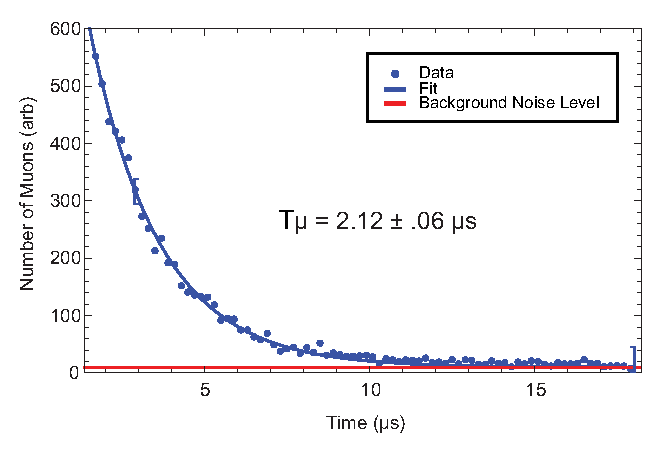
\includegraphics[height=70mm]{./figures/muon_decay.eps}
\caption{A histogram of muon lifetimes. The lifetimes follow exponential decay to some background noise level.  The data was fit using 2-parameter nonlinear regression using $\sqrt{N}$ weighting and excluding the first $2.0~\mu$s.  The fit has an $r^{2}$ value of $.996$ and produces a $\tau_{\mu}$ of $2.12 \pm .06~\mu$s.}
\label{fig:muondecay}
\end{center}
\end{figure}

 As a decay process with some time time constant, $\tau_{\mu}$, we
would expect the data to be modeled by the exponential decay of Equation \eqref{expdecay}.  However because there is background noise recorded by our
scintillator the data is modeled by

\begin{equation}
\label{eq:fitdecay}
N(t) = N_{0} e^{-t/\tau_{\mu}}+b
\end{equation}

where $b$ is the constant background noise level measured by the scintillator. 

To determine the muon mean lifetime, $\tau_{\mu}$, we then fit the
data to Equation~\eqref{eq:fitdecay}.  Fitting involved three major processes: the
determination of the background noise level, $b$, determination of the
fitting range, and finally the determination of the muon mean lifetime
through using a 2-parameter nonlinear regression test based on Equation~\eqref{eq:fitdecay}.

To determine the noise background, a linear regression test was used.
We created an algorithm which iteratively tested increasingly large
portions of the tail end data from Figure~\ref{fig:muondecay} until we detected a
slight correlation ($p$-value $\leq .1$) between the points.  We took
this portion of noncorrelated tail end data to be the result of
background noise measured by the scintillator.  Accordingly, the mean
value of this subset was taken to be the background noise level,
$b$. From our data we determined the background noise level to be 10
events.

Determining the range over which we would fit the data to our model
was a crucial step in determining the mean lifetime of muons.  We
determined that the chance of data corruption increased for smaller
time values due to uncontrollable systematic
limitations (See Appendix \ref{muontimeerroranalysis}). Likewise, we found that the goodness of our fit worsened as
we excluded an increasing amount of front end data points (most likely
due to the exclusion emphasizing the background noise dominating the
tail end data).  Resultantly, we determined that there existed an
optimal range over which to fit.  This range included data with time
values $t \geq t_{c}$, where $t_{c}$ is the cutoff time.  All data
points before and including $t_{c}$ were excluded from the fitting
process.  To determine $t_{c}$, we created an algorithm which
iteratively fit the data with increasing $t_{c}$ using a 2-parameter
nonlinear regression test.  For each fit, the $\tau_{\mu}$ and the
associated $r^{2}$ value were computed for $t_{c}\leq 5~\mu$s.  These
results are shown in Figure~\ref{fig:rsq}.  We wanted $t_{c}$ to be a
value which corresponded to an $r^{2} \geq .995$ and a region of
minimally fluctuating $\tau_{\mu}$.  Observing the Figure~\ref{fig:rsq}, we decided
that $.4~\mu$s$ \leq t_{c}\leq 2.0~\mu$s was an adequate range for $t_{c}$.
Because data for smaller time values were more likely to be corrupted,
we ultimately chose our cutoff time to be $2.0~\mu$s.


\begin{figure}[htbp]
\begin{center}
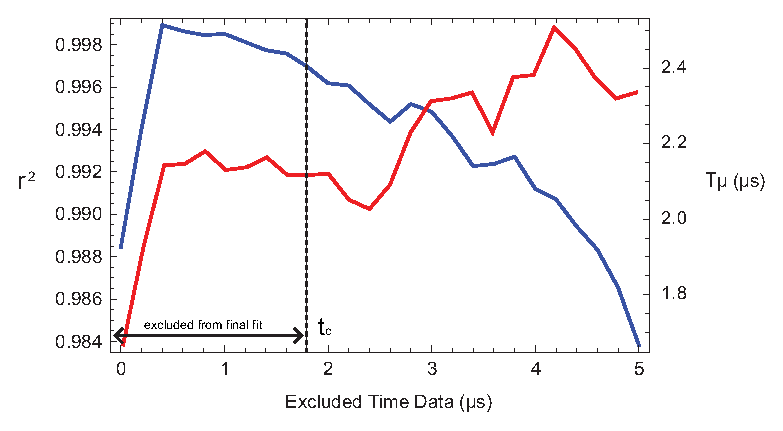
\includegraphics[height=60mm]{./figures/lifetime_fit_param.eps}
\caption{This plot shows the effect of excluding data up to some cutoff time $t_{c}$ from the fitting process.  We chose $t_{c}$ to be $2.0~\mu$s because it produced a value for $\tau{\mu}$ that was in a range of relative stability and because it produced a fit with an $r^{2}$ value $> .995$ as seen above.}
\label{fig:rsq}
\end{center}
\end{figure}

Excluding all points prior to and including $t_{c}$, we were able to determine $\tau_{\mu}$ to be $2.12 \pm 0.16~\mu$s.  This value deviates from the accepted value, $2.20~\mu$s, by $3.8\%$.  However our $7.6\%$ error includes the accepted value.






\subsection{Determination of Muon Mass}\label{determinationofmuonmass}

By measuring the heights of pulses produced by PMT flashes, we are
able to ultimately determine the muon mass.  As discussed in Section
\ref{muonmass}, we can determine this mass by observing the electron cutoff energy, $E_{e}^{max}$. In order to measure electron energy in general
we first calibrated the PMT pulse height to the energy deposited in
the scintillator as discussed in Section \ref{energycalibration}. This calibration
was done by measuring the pulse heights of muon which passed through
all three scintillator panels.  More $50000$ events were observed in
roughly four hours of data aquisition.  The distribution of binned
pulse heights is shown in Figure~\ref{fig:pulseheights}(a).  As previously stated, the
maximum, or the mode, of this distribution corresponds to a minimum in
the Bethe-Block equation (see Appendix \ref{minimumionizationenergy} for more information).  From this we determined that a pulse
height $V_{\mu} = 9.8\pm0.5 \times 10^{-2}$ V corresponds to a $\frac{dE}{dx}= 1.85\pm0.10$ MeV
g$^{-1}$ cm$^{2}$.  Knowing both the density and the thickness of the
scintillator panels to be $2.5\pm0.2$ and $1.08\pm0.09$ g cm$^{-3}$ respectively, we can determine
the actual scale between pulse height and deposited energy.  Taking
this scale to be approximately linear in this regime, we found that
$1$V produced by the PMTs as measured by an oscilloscope, maps to an
energy of $51 \pm 7$ MeV.



\begin{figure}[htbp]
\begin{center}
\subfigure[Histogram of muon pulse heights]{\label{fig:edge-a}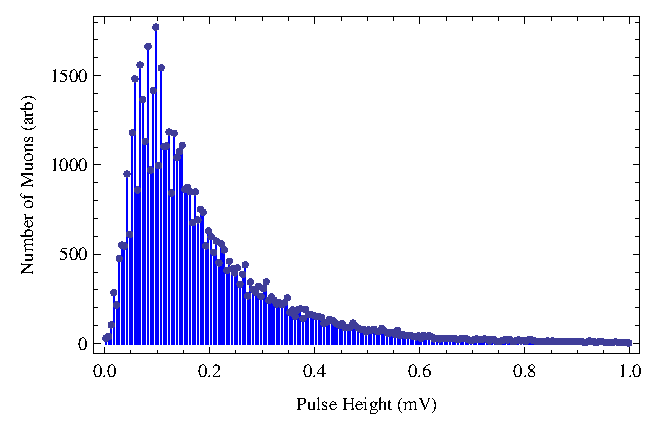
\includegraphics[height=52mm]{figures/Muon_Pulse_Height.eps}}
\hspace{-1mm}
\vspace{-2mm}
\subfigure[Histogram of electron pulse heights]{\label{fig:edge-b}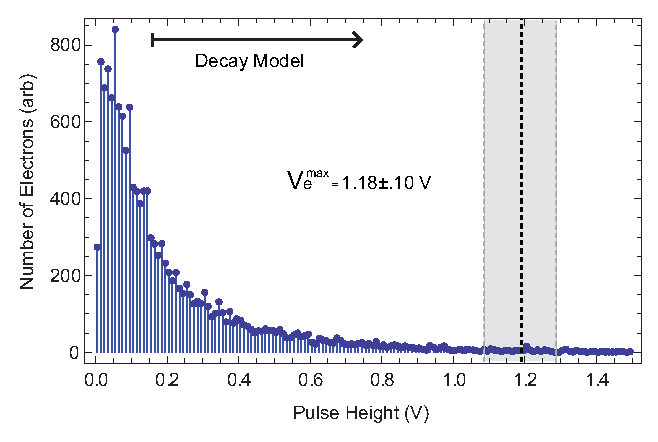
\includegraphics[height=52mm]{figures/Electron_Energy_Cutoff.eps}}
\vspace{-2mm}
\caption{These raw pulse heights produced by the PMTs correspond to muon and electron energies deposited in the scintillators.  Data from (a) is used to calibrate a scale from pulse height (measured in V) to energy (measured in MeV).  Data from (b) was used to determine the electron cutoff energy.  Together information from both plots were used to calculate the muon mass.}
\label{fig:pulseheights}
\end{center}
\end{figure}


By observing the pulse heights produced by PMT flashes from the middle
scintillator that correspond to STOP pulses, we then measured the
energy deposited by electrons produced from muon decay.  This data was
recorded for roughly five days and included nearly $7000$ events.  The
distribution of binned electron pulse heights, $V_{e}$, is shown in
Figure~\ref{fig:pulseheights}(b).  As noted in Section \ref{muonmass}, the shape of this energy
distribution is determined by the kinematics of the muon decay.  Most
importantly, the energy cutoff (the point at which the distribution
decays to zero) occurs at roughly one-half the mass of the decayed
muon.




To determine the energy cutoff of the distribution in Figure~\ref{fig:pulseheights}(b), we
used a fitting algorithm.  First we assumed that after some pulse
height, the distribution could be approximately modeled by an
exponential decay.  To determine this value we did an $r^{2}$ analysis
of multiple fits to using 2-parameter nonlinear regression in which we
excluded an increasingly large range of low pulse heights points
beginning at $V_{e}=0$.  In these fits we weighted each data point by
$\sqrt{N_{e}}$, where $N_{e}$ is the number of electrons in some pulse
height bin.  We determined that the smallest exclusion range to
produce a fit with $r^{2}\geq.99$ was the exclusion range $0$ V $\leq
V_{e}\leq .1$ V.  We were then able to compute the model for the
decay distributions decay as $V_{e}$ approached the cutoff energy.
This model approximated the number of electrons one would expect to
see (relative to the number of events observed, which was nearly 7000)
for some $V_{e}$ .

The model for the distribution's decay was then used to determine
$E_{e}^{max}$ by finding the scope voltage at which the interval
$N_{e}\pm \delta N_{e}$ ($1-\sigma$ error bars) was completely below
$1$.  Because $N_{e}$ is a discrete value being modeled by exponential
decay, we claim that an $N_{e} \leq 1$ essentially corresponds to no
events.  Therefore we take this $V_{e}$, found to be $1.18\pm.10$ V,
to be $V_{e}^{max}$. We take all subsequent nonzero values of $N_{e}$
to be background noise produced by PMT false flashes.  Converting from
$V_{e}^{max}$, we find that $E_{e}^{max}=60.8 \pm 11.1$ MeV.  Based on
the kinematics of the muon decay we determined that this cutoff energy
implies a muon mass of $m_{\mu} = 120 \pm 20$ MeV/c$^{2}$.  This
value deviates from the accepted value, $105.66$ MeV/c$^{2}$, by $12\%$.
However our $17\%$ error includes the accepted value.

\subsection{Determination of the Fermi Coupling Constant}\label{determinationofweakforcecouplingconstant}

Having determined the parameters for both the muon mean lifetime, $\tau_{\mu}$, and the muon mass, $m_{\mu}$ we can calculate the value for $G_{F}$ using Equation \eqref{gf}. Ultimately, from our results we calculate that $G_{F}=3.0\pm1.3\times 10^{-59}$ J m$^{3}$.  This value deviates from the accepted value, $4.305\times10^{-59}$ J m$^{3}$\cite{pdg}, by $43\%$. Our $43\%$ error just includes this accepted value.

Our calculation of $G_F$ is by no means a precision measurement.  Although certain aspects of this experiment have relatively low error ($<8\%$), such as the measurement of $\tau_{\mu}$, ultimately the overwhelming error associated with the energy calibration prevented a more precise measurement of $G_F$.
